\documentclass{beamer}


\usepackage[utf8]{inputenc}
\usepackage{amsmath}
\usepackage{amsfonts}
\usepackage{amssymb}
\usepackage{graphicx}
\usepackage{ragged2e}  % `\justifying` text
\usepackage{booktabs}  % Tables
\usepackage{tabularx}
\usepackage{tikz}      % Diagrams
\usetikzlibrary{calc, shapes, backgrounds}
\usepackage{amsmath}
\usepackage{amssymb}
\usepackage{dsfont}
\usepackage{url}       % `\url
\usepackage{listings}  % Code listings
\usepackage[T1]{fontenc}
\usepackage{subcaption} 


\usepackage{theme/beamerthemehbrs}

\author[]{Abhishek Padalkar}

\title{Dynamic Motion Primitives}
\subtitle{Research and Development Project}
\institute[HBRS]{Hochschule Bonn-Rhein-Sieg}
\date{\today}
\subject{Test beamer}

% \thirdpartylogo{path/to/your/image}


\begin{document}
	{
	\begin{frame}
	\titlepage
	\end{frame}
	}
	
	\begin{frame}{Motivation}
		\begin{itemize}
			\item Humans \textbf{learn} variety of motions and use them in similar situations. 
			\item Human motions consist of motion primitives. 
			\item Concept of motion primitives can be adopted for robots. 
			\item Learned motion primitives can be combined to do complex task. 
			\item Several approaches are available for learning motion primitives.
		\end{itemize}
	\end{frame}
	
	
	\begin{frame}{Advantages of DMP}
		\begin{itemize}
			\item It is a model free learning approach.
			\item Any arbitrary trajectory can be learned in end-effector space as well as in joint space.
			\item Here learning is linear regression, so it does not need large dataset.
			One trajectory is sufficient ideally.
			\item Trajectories can be scaled in space as well as in time.
			\item Trajectory evolves as robot actually moves along the trajectory. Hence on-line modifications in the trajectory are possible.

		\end{itemize}
	\end{frame}

	\begin{frame}{Formulation of DMP}
		\begin{equation}\label{DMP_1}
		\color{blue}\tau\dot{z} = \alpha_{z}(\beta_{z}(g - y) - z) + \color{red}f(x) \color{black}
		\end{equation}
		\begin{equation}\label{DMP_2}
		\color{blue}\tau \dot{y} = z \color{black}
		\end{equation}
		\begin{equation}\label{forcing_term}
		f(x) = \frac{\sum_{i=1}^{N}\psi_{i}(x)w_{i}}{\sum_{i=1}^{N}\psi_{i}(x)}x(g - y_{0})
		\end{equation}
		where,
		\begin{equation}\label{psi}
		\psi_{i} = \exp(-{\frac{1}{2\sigma_{i}^{2}}(x - c_{i})^{2}})
		\end{equation}
		and,
		\begin{equation}\label{canonical}
		\tau \dot{x} = -\alpha_{x}x
		\end{equation}
		\footnote{Formulation of DMP taken from \cite{ijspeert2013dynamical}}
	\end{frame}
	
	
	\begin{frame}
		\begin{itemize}
			\item Second order differential equation representing \textbf{damped mass spring system.} 
			\item Non-linear term \color{red} \textit{f(x)} \color{black} modifies the acceleration and hence characterizes the motion. 
			\item \color{red} \textit{f(x)} \color{black} is normalized weighted sum of equally spaced Gaussian functions. 
			\item Learning a motion primitive means learning the wights 	\textbf{\textit{$w_{i}$}}.
			\item Phase variable \textbf{x} ensures the synchronization between multiple degrees of freedom.  
		\end{itemize}
	\end{frame}

	\begin{frame}{Working of DMP}
		\centering
		\textbf{2D DMP system with no forcing term}
		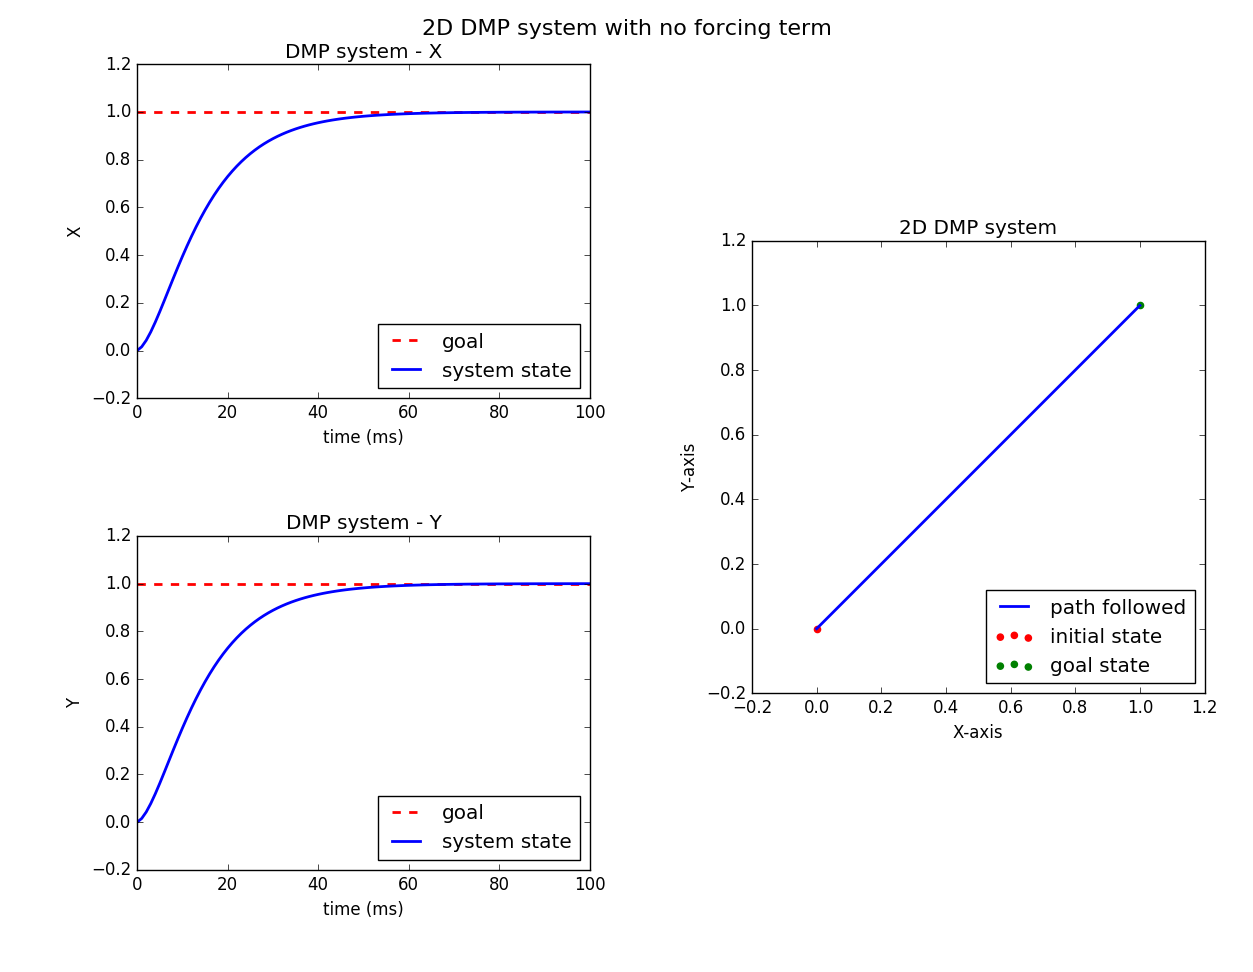
\includegraphics[scale=0.3]{images/dmp_no_f}
	\end{frame}
	
	\begin{frame}
		\begin{figure}
			\begin{subfigure}[b]{0.38\linewidth}
				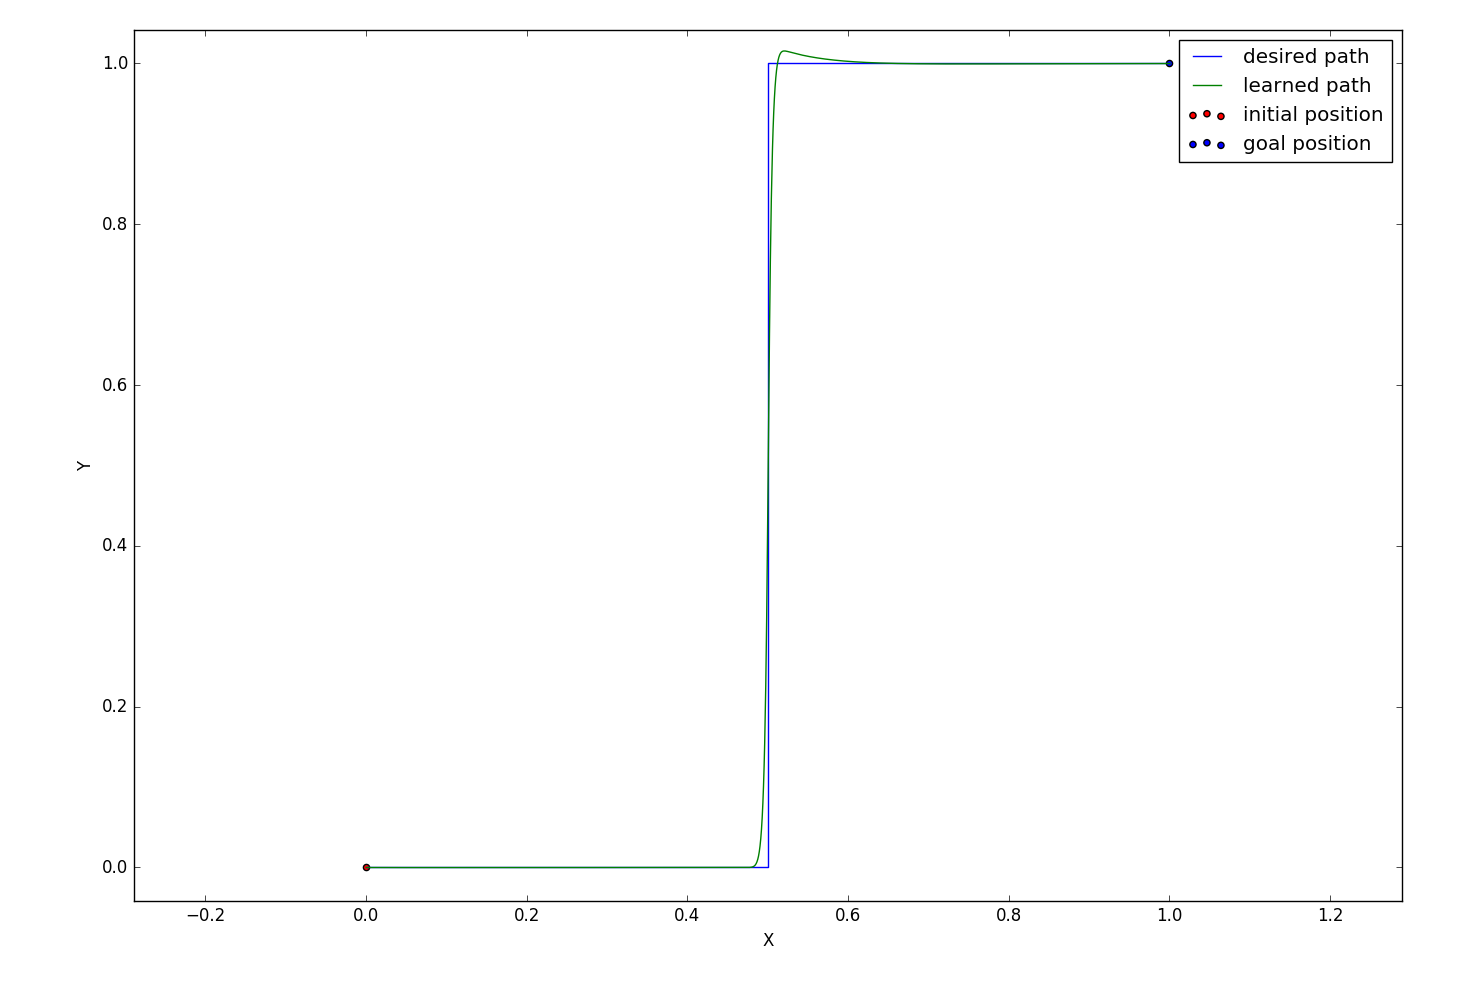
\includegraphics[scale=0.15]{images/step_f.png}
			\end{subfigure}
			\begin{subfigure}[b]{0.60\linewidth}
				\begin{figure}
					\begin{subfigure}[b]{0.5\linewidth}
						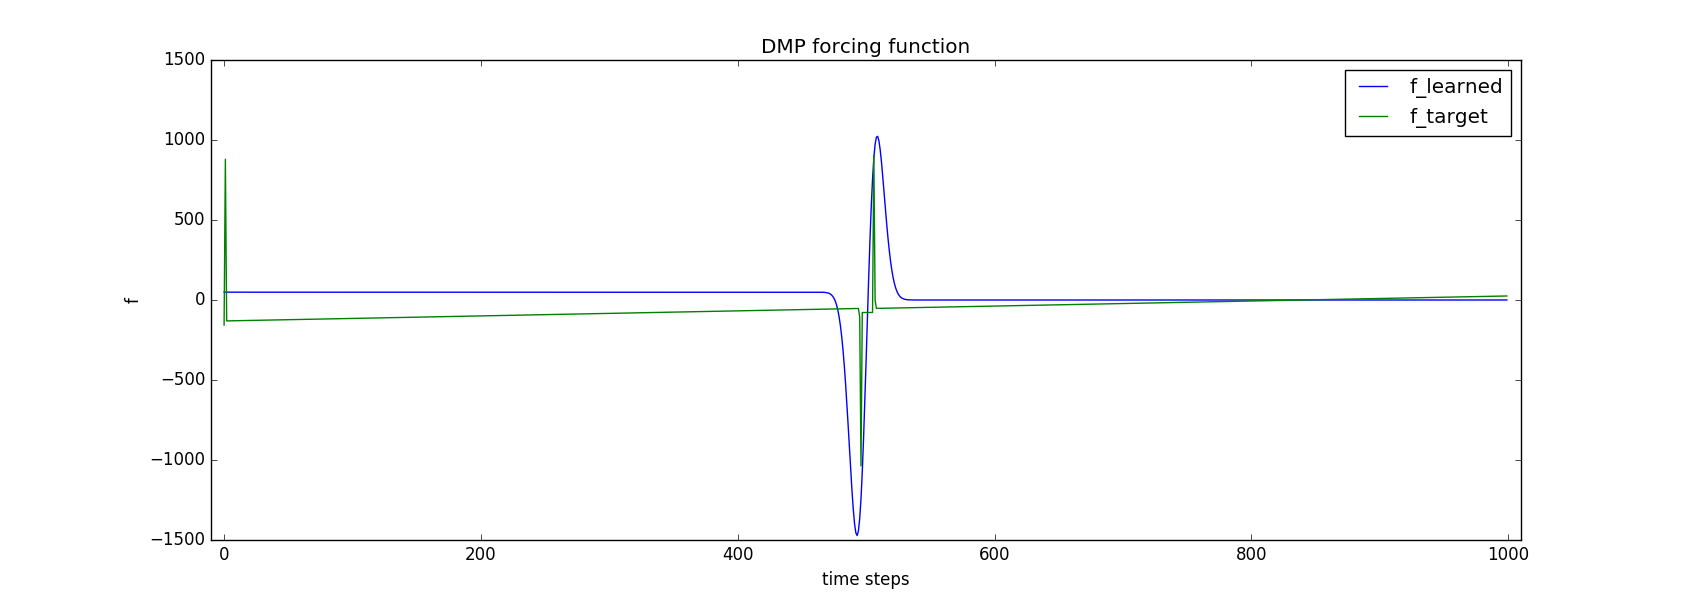
\includegraphics[scale=0.15]{images/f_x.png}
					\end{subfigure}
					\begin{subfigure}[b]{0.5\linewidth}
						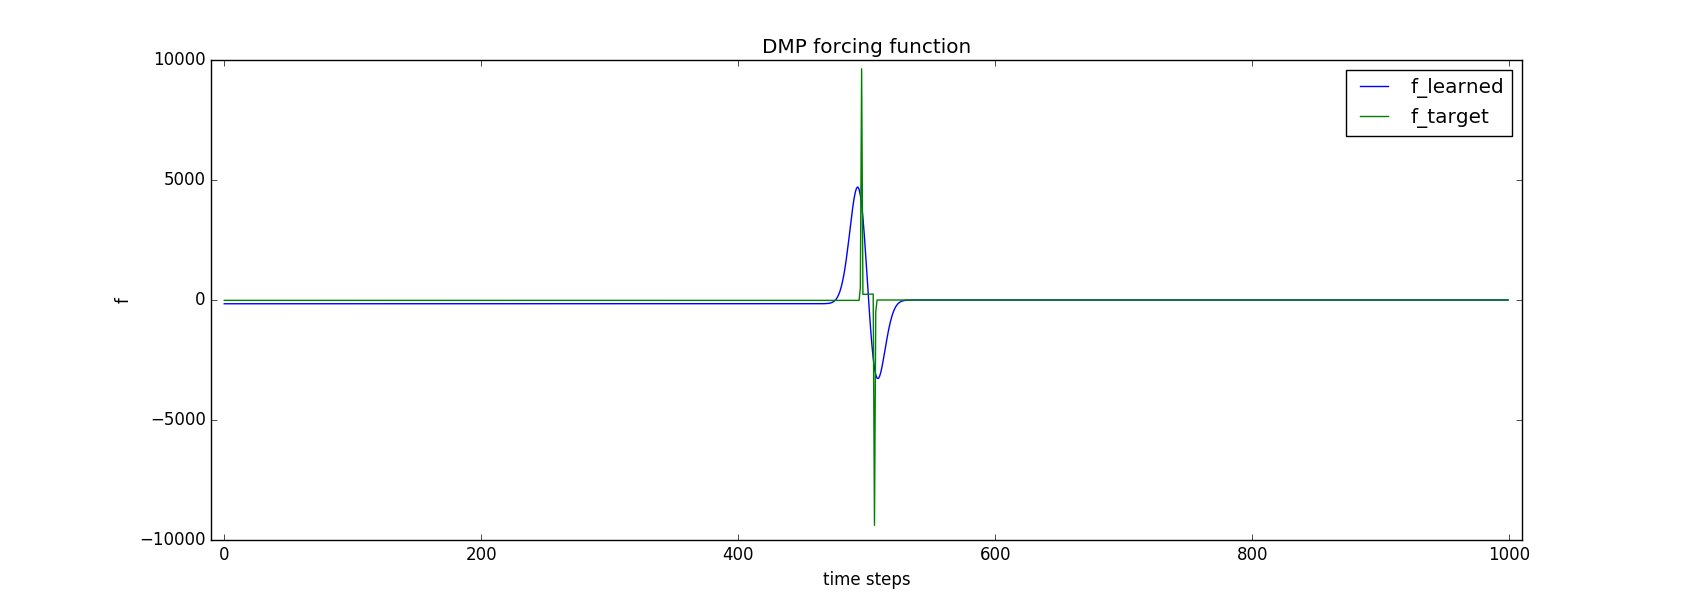
\includegraphics[scale=0.15]{images/f_y.png}
					\end{subfigure}	
				\end{figure}

			\end{subfigure}	
		\end{figure}
	\end{frame}
	

	\begin{frame}{Analysis of the effects of the parameters used in DMP}
		Effect of the number of basis functions on the trajectory approximation
		\begin{center}
			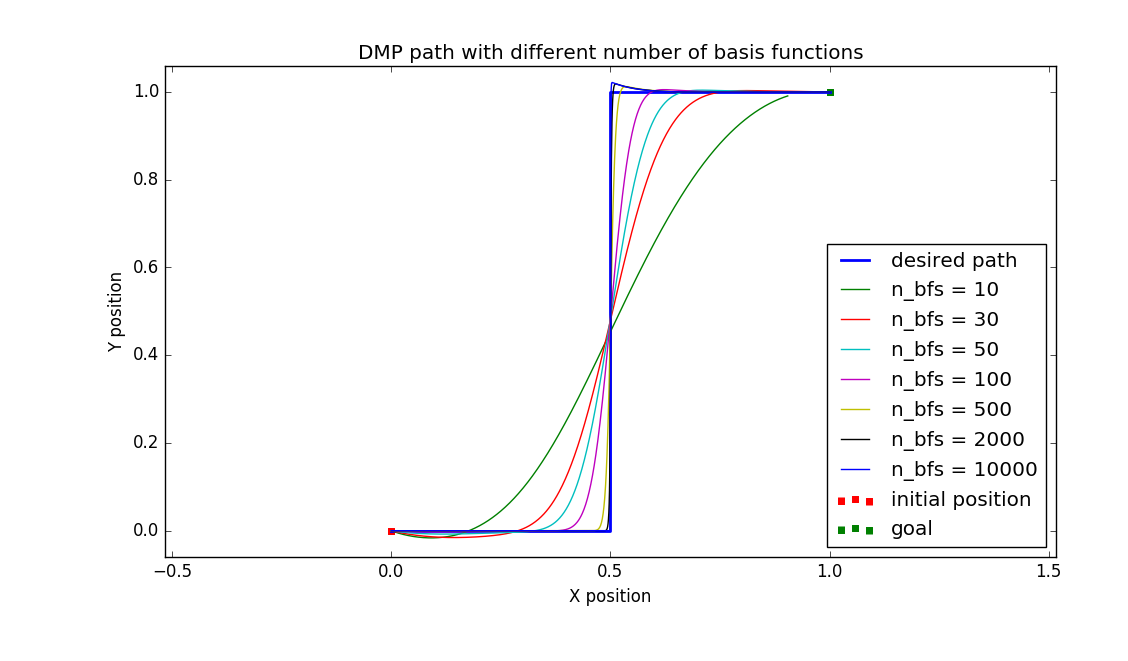
\includegraphics[scale=0.25]{images/n_bfs_}
		\end{center}
		\begin{equation}
		f(x) = \frac{\sum_{i=1}^{\color{red}N\color{black}}\psi_{i}(x)w_{i}}{\sum_{i=1}^{\color{red}N\color{black}}\psi_{i}(x)}x(g - y_{0})
		\end{equation}
	\end{frame}
	
	\begin{frame}
		\textbf{Error in mimicking the trajectory}
		\begin{center}
			\begin{table}[H]
				
				\begin{tabular}{| c | c | c | c | c | c | c | c |}	
					\hline
					n\_bfs & 10 & 30 & 50 & 100 & 500 & 2000 & 10000\\       
					\hline
					Error & 0.093 & 0.038 & 0.021 & 0.009 & 0.002 & 0.001 & 0.001\\
					\hline
				\end{tabular}
				\caption{Error in mimicking the trajectory}
			\end{table}\label{_n_bfs_e}
		\end{center}
		\begin{itemize}
			\item Higher number of basis functions results in better approximation
			\item More number of basis functions learn more noise
		\end{itemize}
	\end{frame}
	
	\begin{frame}
		Effect of the time step on the trajectory approximation
		\begin{center}
			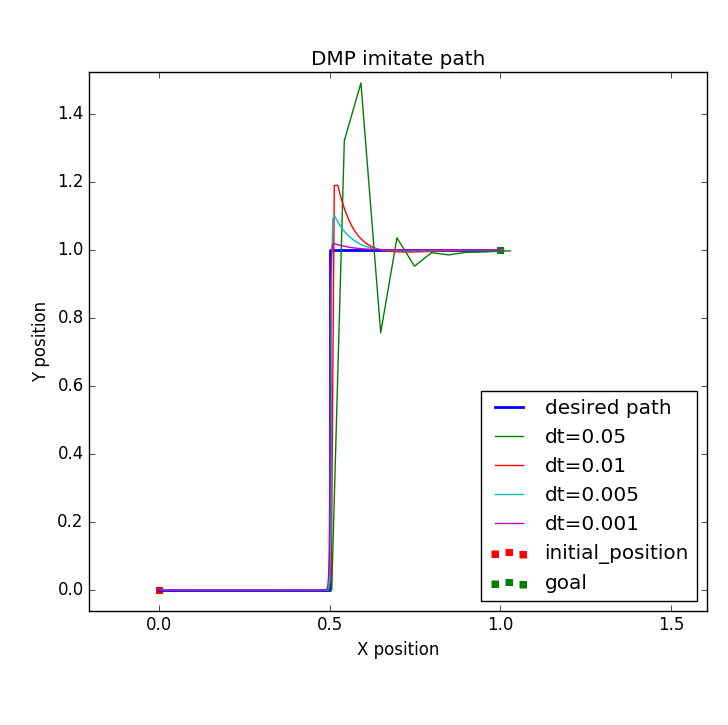
\includegraphics[scale=0.45]{images/dt_}
		\end{center}
	\end{frame}
	
	\begin{frame}
		Effect of the time step on the trajectory approximation
		\begin{center}
			\begin{table}[H]
				\centering
				\begin{tabular}{| c | c | c | c | c | c | c | c |}	
					\hline
					Time step size & 0.05 & 0.01 & 0.005 & 0.001 \\       
					\hline
					Error & 0.062 & 0.017 & 0.011 & 0.007 \\
					\hline
				\end{tabular}
				\caption{Error in mimicking the trajectory}
			\end{table}\label{_dt_e}
		\end{center}
	\end{frame}
	
	
	\begin{frame}
		Effect of the time scaling factor on the trajectory approximation
		\begin{center}
		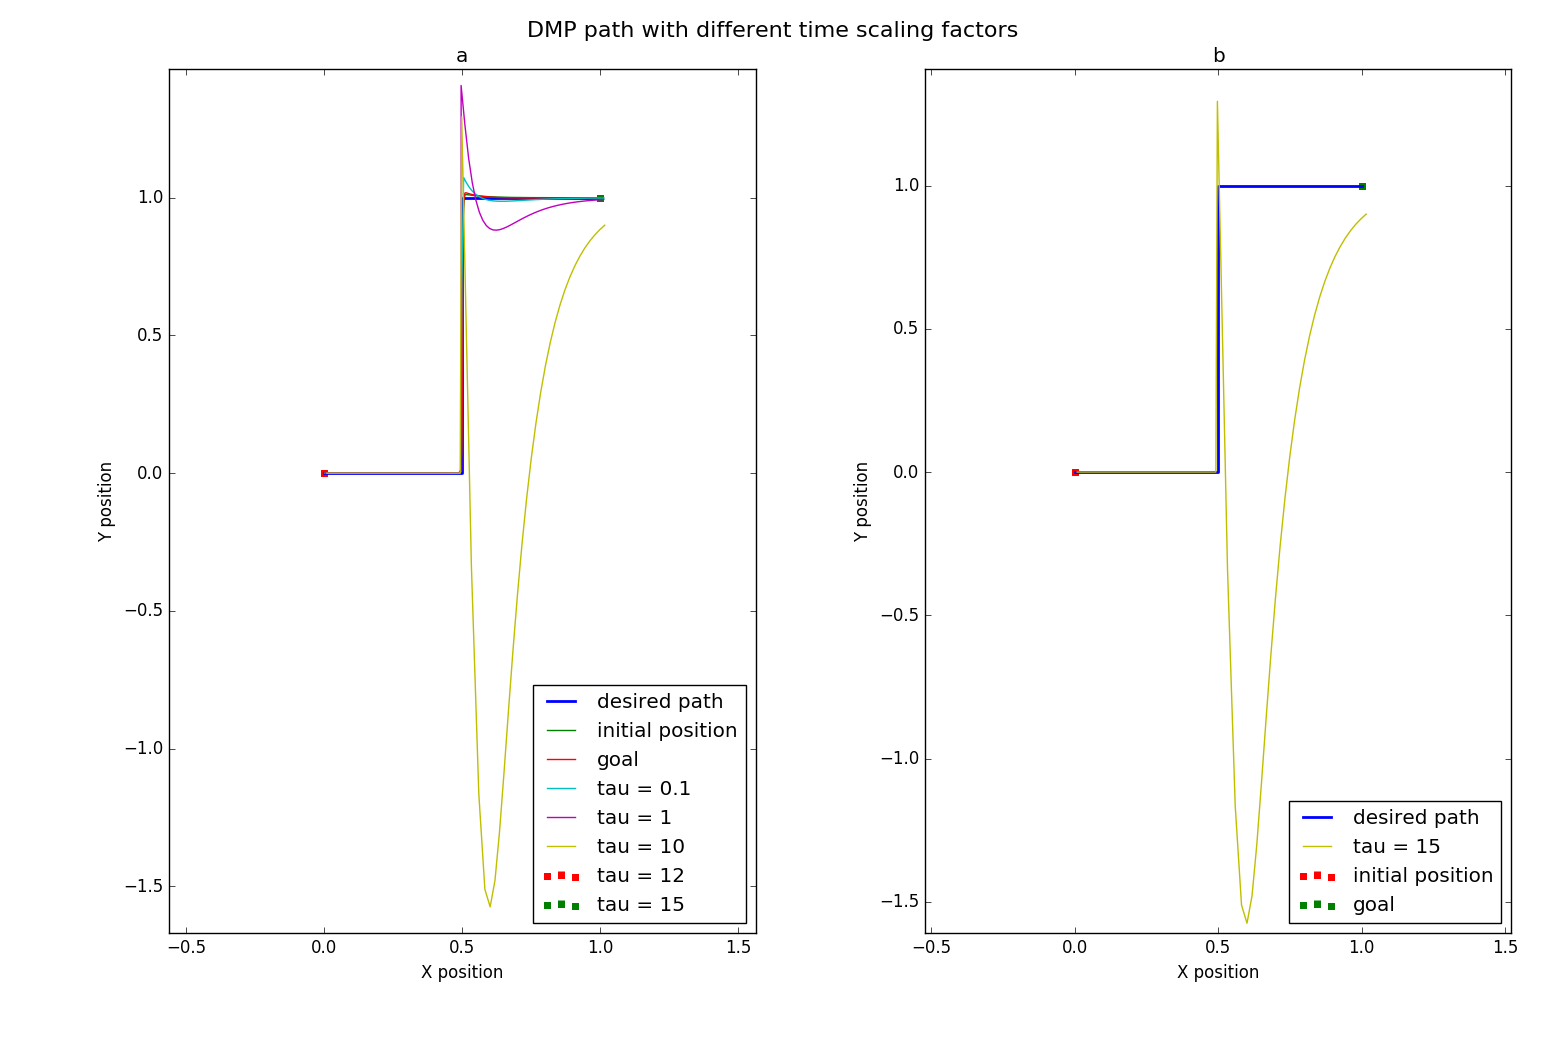
\includegraphics[scale=0.24]{images/tau_}
		\end{center}
		\begin{equation}
		\color{red}\tau \color{black}\dot{z} = \alpha_{z}(\beta_{z}(g - y) - z) + f(x)
		\end{equation}
		\begin{equation}
		\color{red}\tau \color{black} \dot{y} = z 
		\end{equation}

	\end{frame}
	
	\begin{frame}
		Effect of the time scaling factor on the trajectory approximation
		\begin{center}
			\begin{table}[H]
				\centering
				\begin{tabular}{| c | c | c | c | c | c | c | c |}	
					\hline
					Time scaling factor ($tau$) & 0.1 & 1 & 10 & 12 & 15 \\       
					\hline
					Error & 0.007 & 0.007 & 0.010 & 0.036 & 0.292   \\
					\hline
				\end{tabular}
				\caption{Error in mimicking the trajectory}
			\end{table}\label{_tau_e}
		\end{center}
	\end{frame}
	
	\begin{frame}{Inverse Kinematic Solver}
		\begin{itemize}
			\item Motion is learned in Cartesian space. 
			\item Need of inverse kinematic solver to convert Cartesian velocity commands to joint velocity commands. 
			\item Limitations of manipulators due to 5 degrees of freedom.
			\item Weighted Damped Least Square method for calculating joint velocities.
		\end{itemize}	
	\end{frame}
	
	\begin{frame}{Whole Body Motion Control}
		\begin{equation}
		m_{cap} = \frac{(\sigma_{min} - \sigma_{l})}{(\sigma_{h} - \sigma_{l})}
		\end{equation}
		
		
		\begin{equation}
		b_{cap} = \frac{(d - d_{l})}{(d_{h} - d_{l})}
		\end{equation}
		
		
		\begin{equation}
		v_{ee} = \frac{m_{cap}}{m_{cap} + b_{cap}}.v
		\end{equation} 
		
		\begin{equation}
		v_{b} = \frac{b_{cap}}{m_{cap} + b_{cap}}.v
		\end{equation} 
	\end{frame}
	\begin{frame}
		Where, \\
		$\sigma_{min}$ is the smallest sigma value, \\
		$\sigma_{l}$ is the lower limit on $\sigma_{min}$, \\
		$\sigma_{h}$ is the upper limit on $\sigma_{min}$, \\
		$d$ is the distance of the obstacle from base, \\
		$d_{l}$ is the lower limit on $d$, \\
		$d_{h}$ is the upper limit on $d$, \\
		$v$ is the desired velocity of end-effector in global frame of reference, \\ 
		$v_{ee}$ is the velocity command for end-effector of the manipulator in global frame of reference, \\
		$v_{b}$ is the velocity command for mobile base in global frame of reference.

	\end{frame}
	
	\begin{frame}{Experiments}
		\begin{itemize}
			\item Experiments were conducted on Kuka YouBot and Toyota HSR to evaluate :
			\begin{itemize}
				\item \textbf{\textit{Learning from Demonstration}} framework
				\item \textbf{\textit{Whole body motion control}}
			\end{itemize}  
			\item Experiments on Kuka YouBot :
			\begin{itemize}
				\item 3 inverse parabolic trajectories 
				\item 1 step function like trajectory 
				\item 1 square function trajectory 
				\item 1 inverse parabolic trajectory (whole body motion)
				\item 2 square wave trajectories (whole body motion)
			\end{itemize}
			\item Experiments on Toyota HSR:
			\begin{itemize}
				\item Sequencing 2 DMPs for pick and place task
				\item Grasping an object
			\end{itemize}
		\end{itemize}
	\end{frame}
	
	\begin{frame}{Results}
		\text{Inverse Parabolic Trajectory}
		\begin{figure}
			\begin{subfigure}[b]{0.49\linewidth}
				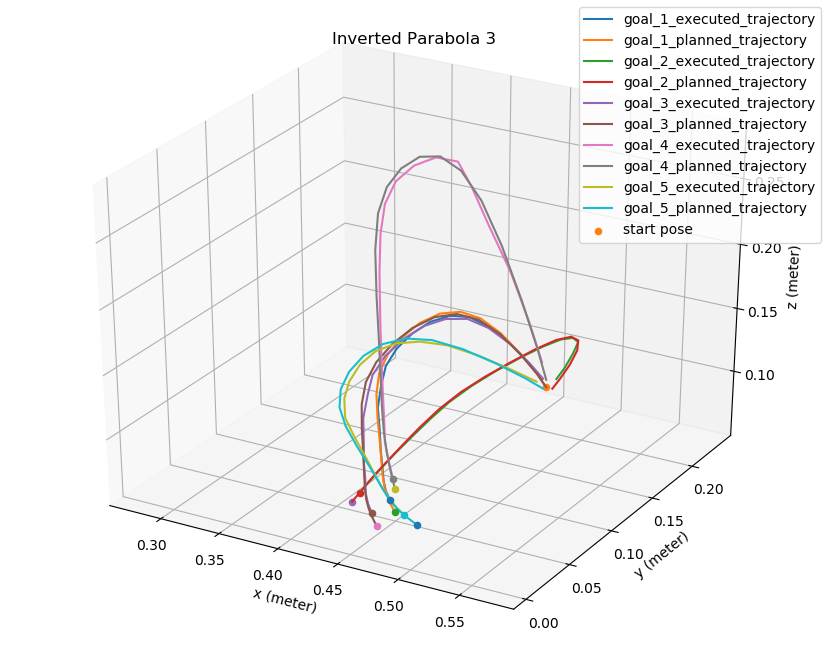
\includegraphics[scale=0.25]{images/1/inv_par_3.png}
			\end{subfigure}
			\begin{subfigure}[b]{0.49\linewidth}
				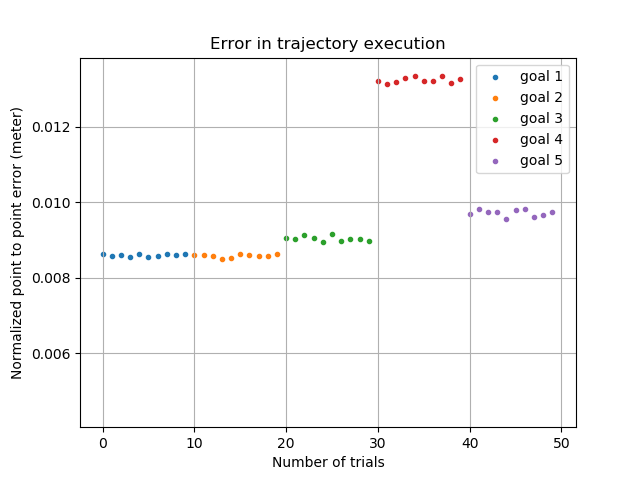
\includegraphics[scale=0.25]{images/1/inv_par_3_e.png}
			\end{subfigure}	
		\end{figure}
	\end{frame}
	
	\begin{frame}{Results}
		Step Function Trajectory
		\begin{figure}
			\begin{subfigure}[b]{0.49\linewidth}
				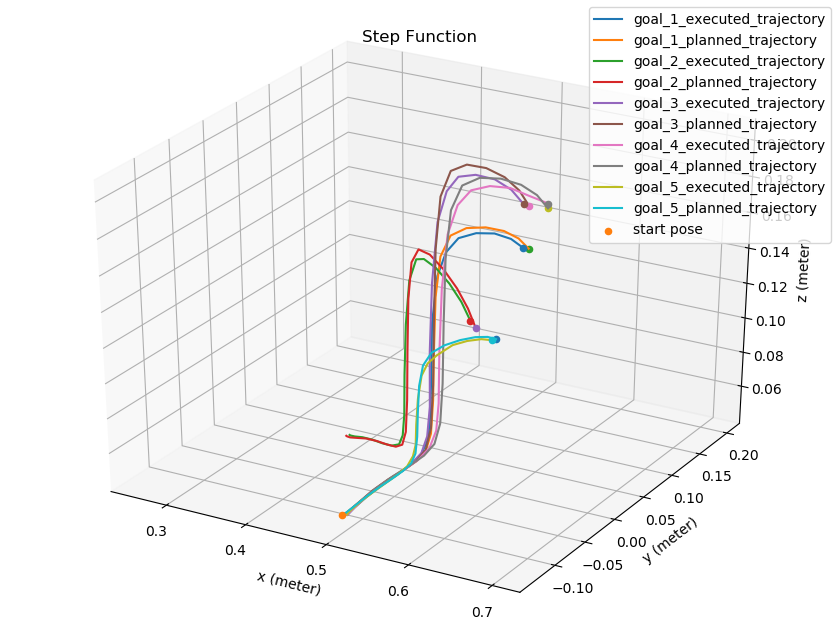
\includegraphics[scale=0.25]{images/1/step.png}
			\end{subfigure}
			\begin{subfigure}[b]{0.49\linewidth}
				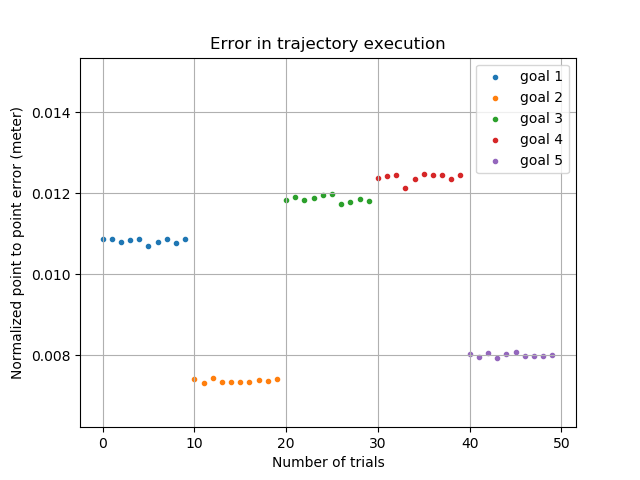
\includegraphics[scale=0.25]{images/1/step_e.png}
			\end{subfigure}	
		\end{figure}
	\end{frame}

		
	\begin{frame}{Results}
		\begin{figure}
			\begin{subfigure}[b]{0.49\linewidth}
				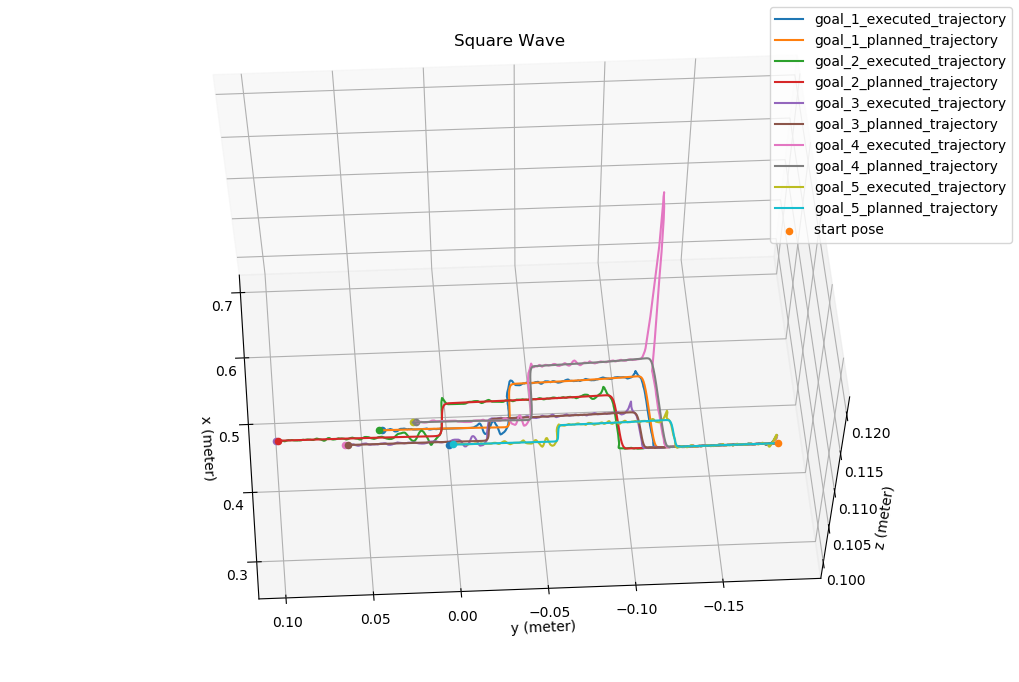
\includegraphics[scale=0.25]{images/1/square.png}
			\end{subfigure}
			\begin{subfigure}[b]{0.49\linewidth}
				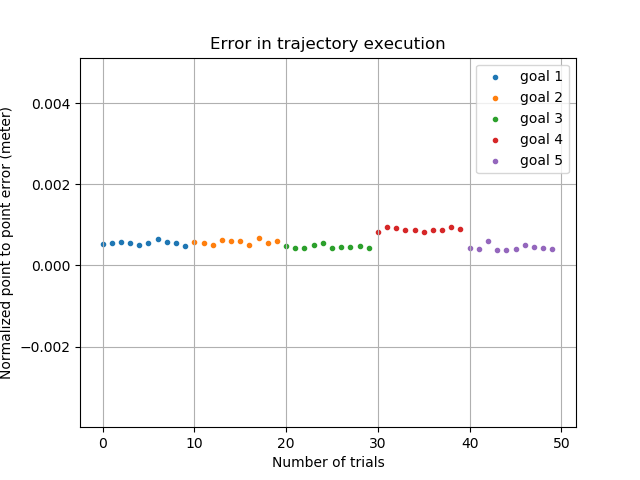
\includegraphics[scale=0.25]{images/1/square_e.png}
			\end{subfigure}	
		\end{figure}
	\end{frame}

		
	\begin{frame}{Results}
		\begin{figure}
			\begin{subfigure}[b]{0.49\linewidth}
				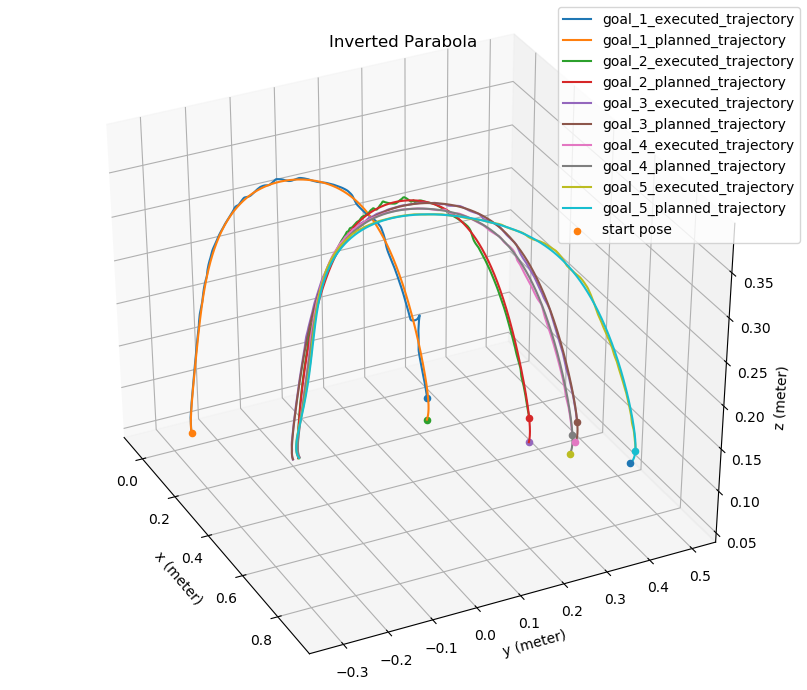
\includegraphics[scale=0.25]{images/2/inv_par.png}
			\end{subfigure}
			\begin{subfigure}[b]{0.49\linewidth}
				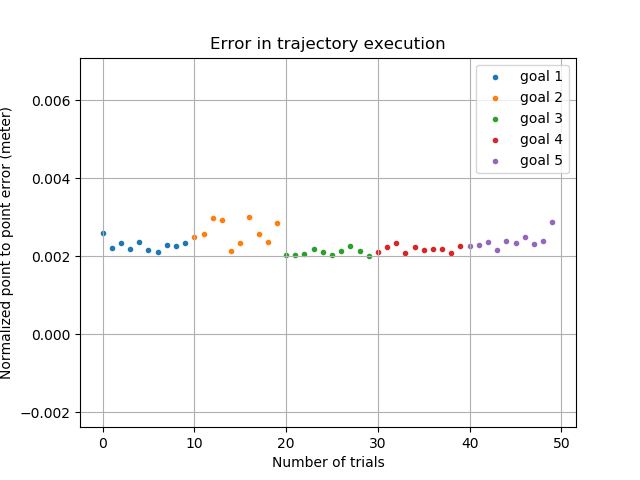
\includegraphics[scale=0.25]{images/2/inv_par_e.png}
			\end{subfigure}	
		\end{figure}
	\end{frame}
	
	
	\begin{frame}{Results}
		\begin{figure}
			\begin{subfigure}[b]{0.49\linewidth}
				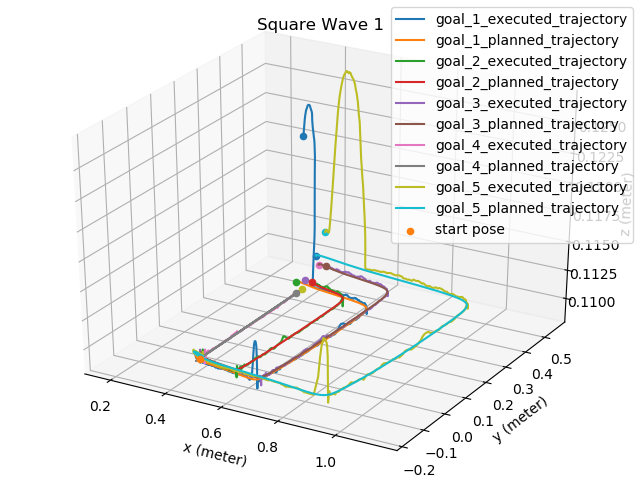
\includegraphics[scale=0.25]{images/2/square.png}
			\end{subfigure}
			\begin{subfigure}[b]{0.49\linewidth}
				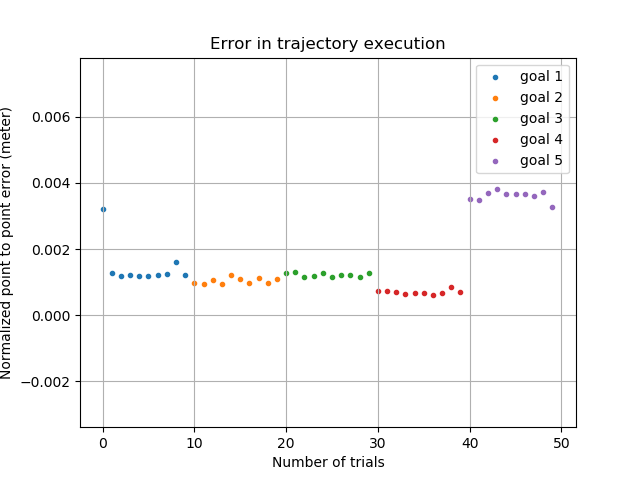
\includegraphics[scale=0.25]{images/2/square_e.png}
			\end{subfigure}	
		\end{figure}
	\end{frame}

	
	\begin{frame}{Results}
		\centering
		Sequencing Two DMPs for object pick and place
		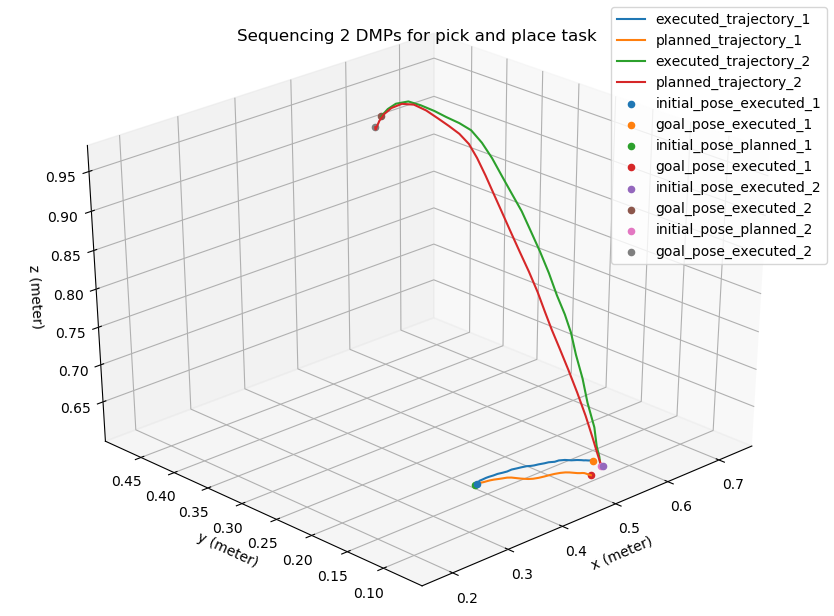
\includegraphics[scale=0.4]{images/HSR_3/sequence.png}
	\end{frame}
	\begin{frame}{Results}
		\begin{figure}
			\begin{subfigure}[b]{0.49\linewidth}
				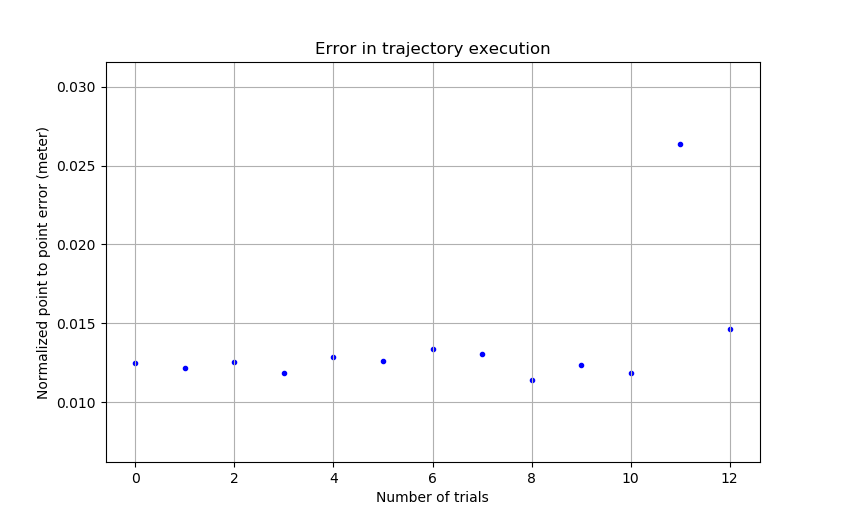
\includegraphics[scale=0.25]{images/HSR_3/sequence_0_e.png}
			\end{subfigure}
			\begin{subfigure}[b]{0.49\linewidth}
				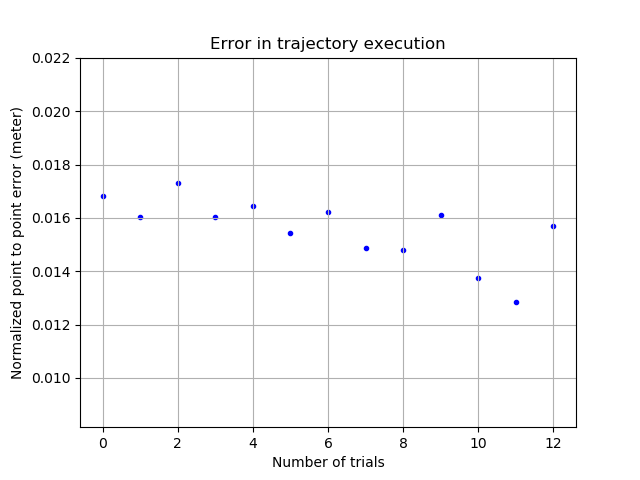
\includegraphics[scale=0.25]{images/HSR_3/sequence_1_e.png}
			\end{subfigure}	
		\end{figure}
	\end{frame}

	\begin{frame}{Conclusion}
	\begin{itemize}
		\item Development of \textit{Learning from Demonstration} framework for robot programming using DMPs.
		\item Analysis of the effects of the parameters used in DMPs on trajectory approximation. 
		\item Evaluation of \textit{Learning from Demonstration} framework on KUKA YouBot and Toyota HSR. 
		\item Development and evaluation of whole body motion control architecture.
		\item Gathering insights of working of DMPs as well as their capabilities and limitations. 
		\item Integration into current software solution for manipulation for Toyota HSR (replacing MoveIt!).
	  	\end{itemize}
	\end{frame}
\addcontentsline{toc}{chapter}{References}
\bibliographystyle{plain} % Use the plainnat bibliography style
\bibliography{bibliography} % Use the bibliography.bib file as the source of references
\end{document}

